\section{GUI}
Det grafiska användargränssnittet har skapats för att underlätta användandet av ENVISIoN.  Detta möjliggör att ENVISIoN kan köras utan att öppna Inviwos användarfönster. 
\subsection{Utseende}
Det grafiska användargränsnittet skall byggas upp av en grupperingsmeny med möjlighet att fälla ut undermenyer. Fönstret öppnas med menyerna infällda. För att fälla ut en meny skall pilen till vänster om rubriken klickas på. Exemplet nedan visar hur parser-menyn hålls infälld medan visualiserings-menyn är utfälld.

\subsection{Pythonberoenden}
Då Pythons standardbibliotek inte innefattar all, till GUI:t, önskad funktionalitet krävs installation och importering av andra bibliotek och moduler. De bibliotek som använts vid utvecklandet är:

\begin{itemize}
    \setlength\itemsep{0em}
    \item H5py
    \item Matplotlib
    \item Numpy
    \item wxPython
\end{itemize}

H5py är det bibliotek som används för läsning och skrivning till hdf5-filer. Det är framförallt parser-systemet som har användning av detta bibliotek. Under utvecklingen av parameterstyrning hos visualiseringar lades styrning av överföringsfunktions-punkter till. I Inviwo kan ett histogram, en widget, åskådliggöras för att se hur volymdatan är distribuerad för att kunna placera dessa punkter relevant. Då denna widget ligger gömd i Inviwo, vilket gör det svårt att utnyttja denna funktionalitet, underlättade ett externt bibliotek visningen av histogram. Matplotlib möjliggör histogram-funktionen genom modulen pyplot. Numpy-biblioteket innehåller bland annat vetenskapliga beräkningar samt behållare för lagring och behandling av data.
Det bibliotek som utgör den stora delen av det utvecklade användargränssnittet är wxPython. 
\subsubsection{wxPython definitioner}
GUI-biblioteket wxPython innehåller ett stort antal klasser och funktioner. Beroende på vilket funktionalitet som vill uppnås implementeras användning av vissa delar av wxPython. De klasser som använts under utvecklingen av ENVISIoN listas nedan\cite{wxPythonDoc}.
\begin{itemize}
    \setlength\itemsep{0em}
    \item \textbf{wx.App: } Klass som möjliggör applikationskörning.
    \item \textbf{wx.Frame: }Klassen för fönstret som det grafiska användargränssnittet finns i.
    \item \textbf{wx.Panel: }Klass som etablerar en del av fönstret där kontroller och element kan placeras.
    \item \textbf{ wx.lib.scrolledpanel.ScrolledPanel: }En panelklass som möjliggör skrollning och automatisk skroll-uppdatering.
    \item \textbf{wx.Sizers: }En abstrakt klass som används för att placera underfönster i huvudfönstret.
    \begin{itemize}
        \item \textbf{wx.BoxSizer: }En underklass till wx.Sizer somhar en enkel geometrisk form.
    \end{itemize}
    \item \textbf{wx.CollapsiblePane: }Detta är en klass för kollapsbara menyer, som expanderar och kollapsar vid musklick.
    \item \textbf{wx.MessageDialog: }Klass för att visa meddelanden för användaren.
    \item \textbf{wx.StaticText: }Klass för att visa fast text i gränssnittet.
    \item \textbf{wx.Button: }Klass för att skapa kanppar och ge dessa funktion vid klick.
    \item \textbf{wx.TextCtrl: }Klass för inmatning och läsning av text.
    \item \textbf{wx.Choice: }Klass för skapande och visande av lista samt möjligheten av välja objekt i lista.
    \item \textbf{wx.ComboBox: }Klass som kombinerar funktioner för wx.Choice och wx.TextCtrl
    \item \textbf{wx.DirDialog: }Klass för att öppna filhanterare och i den välja en mapp.
    \item \textbf{wx.FileDialog: }Klass för att öppna filhanterare och i den välja en fil av viss filtyp.
    \item \textbf{wx.Slider: }Klass för att skapa skjutreglage.
    \item \textbf{wx.CheckBox: }Klass för att skapa kryssrutor med på/av alternativ.
    \item \textbf{wx.ColourPickerCtrl: }Klass för att välja färg genom ett separat fönster med färgskalor.
    \item \textbf{wx.Colour: }Färgklass med RGB-värde som innehåll.
    \item \textbf{wx.Size: }Storleksklass med pixelstorlek i höjdled och bredd.
    \item \textbf{wx.LogError: }Inbyggd felhantering i wxPython.
    \item \textbf{Event-hantering: }Hantering av händelser i GUI:t, såsom knapptryck, reglageändringar och textändringar.
    \begin{itemize}
        \setlength\itemsep{0em}
        \item \textbf{Bind-funktionen: }
        \item \textbf{wx.EVT\_COLLAPSIBLEPANE\_CHANGED: }Signal som skickas av wx.CollapsiblePane vid kollaps eller expansion.
        \item \textbf{wx.EVT\_BUTTON: }Signal som skickas av wx.Button vid knapptryck.
        \item \textbf{wx.EVT\_TEXT\_ENTER: }Signal som skickas av textfälten då enter-knappen trycks på tangentbordet.
        \item \textbf{wx.EVT\_COMBOBOX: }Signal som skickas av wx.ComboBox när objekt i lista väljs.
        \item \textbf{wx.EVT\_TEXT: }Signal som skickas av wx.TextCtrl när texten ändras i rutan.
        \item \textbf{wx.EVT\_SLIDER: }Signal som skickas av wx.Slider när reglaget flyttas.
        \item \textbf{wx.EVT\_CHOICE: }Signal som skickas av wx.Choice när ett objekt väljs i listan.
        \item \textbf{wx.EVT\_KILL\_FOCUS: }Signal som skickas när ett objekt tappar fokus.
        \item \textbf{wx.EVT\_COLOURPICKER\_CHANGED: }Signal som skickas när en färg har valts i färgnateringsfönstret.
    \end{itemize}
\end{itemize}


\subsection{Översikt över gränssnittet}
När ENVISIoN-applikationen körs öppnas det grafiska gränssnittet. I figur \ref{fig:Startup} visas hur GUI:t ser ut i Windows och i Linux vid start.

\begin{figure}[H]
  \centering
    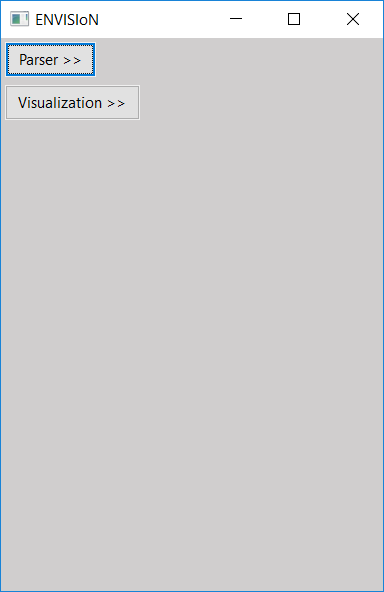
\includegraphics[scale=0.5]{images/GUI/GUIBasWin.png}
    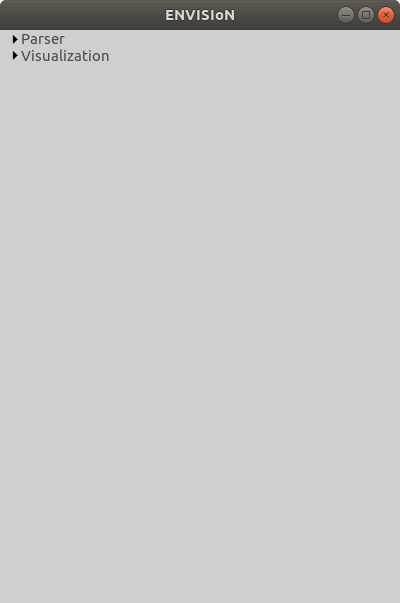
\includegraphics[scale=0.49]{images/GUI/GUIBasLinux.png}
    \caption{Startläge för ENVISIoN, Windows till vänster och Linux till höger.}
    \label{fig:Startup}
\end{figure}

GUI-t är utvecklat som en wx.App. Denna klass har en wx.Frame, vilket är hela det fönstret som visas. Detta fönster har i sin tur en wx.lib.scrolledpanel.ScrolledPanel vilket är en panel som möjiggör skrollning och att placera objekt och lägga till underfönster i GUI:t. I fönsterklassen finns även två kollapsbara menyer för parsning och visualisering. Det är dessa två som är synliga i figur \ref{fig:Startup}.

I appendix A illustreras sökvägarna, utgående från toppmappen $ENVISIoN$ till de filer som är relevanta för GUI:t.

\subsection{Hjälpklasser}
Det finns många likheter mellan vad som ska styras från gränssnittet mellan de olika visualiseringarna. För att abstrahera koden och för att minska kodupprepning så har vissa klasser skrivits som kan användas till olika visualiseringsmenyer.

\subsubsection{GeneralCollapsible}
För att skapa de kollapserbara menyerna som gränssnittet i stor del bygger på så har en klass skapats för det kallad \textit{GeneralCollapsible}. Klassen ärver wxPythons \textit{wx.CollapsiblePane} och får mycket av sin funktionalitet därifrån, men funktioner har lagts till för att kunna bygga strukturer där kollapserbara menyerna har egna kollapserbara menyerna under sig. 

Klassen används aldrig direkt utan ärvs istället av andra klasser som använder sig av den för att bygga upp sin del av gränssnittet.

\newpage

Viktiga funktioner:
\begin{itemize}
    \setlength\itemsep{0em}
    \item \textbf{add\_item: } Funktionen används för att lägga till en godtycklig wxPython-widget under menyns sizer. Notera att denna funktion inte ska användas för att lägga till \textit{GeneralCollapsible}-element. 
    \item \textbf{add\_sub\_collapsible: } Används för att lägga till ett annan instans av en \textit{GeneralCollapsible} klass under menyn.
    \item \textbf{on\_collapse: } Funktionen som kallas då man fäller ut eller in menyn. Det enda funktionen gör är att kalla på \textit{update\_collapse}-funktionen. Funktionen kan overridas i subklasser men det är då viktigt att även de kallar på \textit{update\_collapse}, annars så uppdateras inte layouten korrekt.
    \item \textbf{update\_collapse: } Denna funktion ser till att alla element fyttas och ändrar storlek korrekt efter att en meny har fällts ut eller in. 
\end{itemize}

\nyBild{GUI/general_collapse_ex.PNG}{GeneralCollapsibles sizer struktur.}{GeneralCollapsible_sizers}{1}
Ett \textit{GenralCollapsible}-objekts form då den är tillagd på ett fönster byggs upp av tre sizer-objekt, som visat i figur \ref{fig:GeneralCollapsible_sizers}. \textit{hBox} är en horisontell sizer som sätts till \textit{wx.CollapsiblePane}s huvudsizer. På denna läggs \textit{fillSizer} och \textit{sizer} till. \textit{fillSizer} Fungerar bara för att fylla ut vänsterkanten så att underobjekt till menyn förskjuts en bit åt höger. \textit{sizer} är den sizer som underobjekt sedan kommer att läggas till på. 

\subsubsection{VolumeCollapsible}
En kollapserbar meny för att styra en volymrenderingsaspekten av en visualisering. Denna används i både laddningstäthets- och i ELF-menyn (och bör även användas till partiell laddningstäthet då den läggs till i gränssnittet).

Klassen interagerar med ett \textit{VolumeNetworkHandler}-objekt för att styra den del av inviwonätverket som är relevant. \textit{VolumeCollapsible} initierar inte sin egen \textit{VolumeNetworkHandler} utan variabeln \textit{networkHandler} måste sättas utifrån klassen innan den kan användas.

\newpage

\textit{VolumeCollapsible} låter en användare göra följande:
\begin{itemize}
    \setlength\itemsep{0em}
    \item Välja \textit{shading mode} för volymrenderingen.
    \item Lägga till och ta bort transferfunktionspunkter med godtyckligt värde, transparens, och färg.
    \item Välja fullständig transparens före den lägsta transferfunktionspunkten.
    \item Visa ett histogram över volymdensitetsdistributionen i den aktiva volymdatan.
    \item Ladda och spara aktiv transferfunktion.
\end{itemize}

\begin{figure}[H]
  \centering
  \begin{minipage}[b]{0.4\textwidth}
    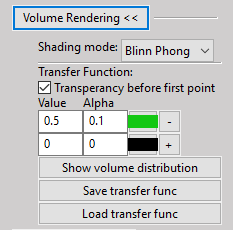
\includegraphics[width=\textwidth]{GUI/volume_collapse.PNG}
    \caption{VolumeCollapsible-objekt i fönster.}
  \end{minipage}
  \hfill
  \begin{minipage}[b]{0.4\textwidth}
    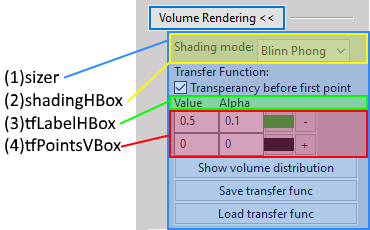
\includegraphics[width=\textwidth]{GUI/volume_collapse_sizers.PNG}
    \caption{VolumeCollapsible, sizer-struktur.}
  \end{minipage}
\end{figure}

\textbf{TFPointWidget: } För att förenkla och abstrahera GUI-strukturen så har en klass TFPointWidget definerats. Widgeten har två \textit{wx.TextCtrl} textfält för att välja värde och transparens för punkten, en \textit{wx.ColourPicker} för att välja färg och en knapp för att ta bort eller lägga till punkter. Klassen interagerar inte direkt med inviwonätverket utan är bara till för att abstrahera GUI-strukturen. Funktioner finns för att hämta ut värden från textfält och färg.

\nyBild{GUI/tf_widget.PNG}{Utseense för en TFPointWidget.}{tf_widget}{1}

Viktiga funktioner i \textit{VolumeCollapsible}:
\begin{itemize}
    \setlength\itemsep{0em}
    \item \textbf{add\_tf\_point: } Lägger till en transferfunktionspunkt i inviwonätverkets raycasterprocessor. Lägger också till ett nytt wx.TextCtrl-element under \textit{tfPointsVBox}-sizern. Binder också callbacks för \textit{TFPointWidget}-objektets events. 
    \item \textbf{remove\_tf\_point: } Tar bort en transferfunktionspunkt i inviwonätverkets raycasterprocessor. Tar bort motsvarande \textit{TFPointWidget}-objektet.
    \item \textbf{update\_tf\_point: } Ändrar en redan existerande transferfunltionspunkt. Detta görs genom att punkten först tas bort och en ny sedan läggs till med uppdaterade värden. Kallas då information i textfälten i någon av de tillagda \textit{TFPointWidget}-objekten ändras.
    \item \textbf{set\_tf\_point\_color} Ändrar färgen för en transferfunltionspunkt. Kallas då färgen ändras i någon av de tillagda \textit{TFPointWidget}-objekten.
    \item \textbf{update\_mask: } Sätter en så kallad \textit{mask} på transferfunktionen så att bara värden över den första transferfunktionspunktetn är synliga.
    \item \textbf{load\_transfer\_function: } Öppnar ett dialogfönster för att välja en fil. Försöker sedan att transferfunktionsdata från den filen. 
    \item \textbf{save\_transfer\_function: } Öppnar ett dialogfönster för att välja en fil. Skriver sedan transferfunktionsdata till den filen.
\end{itemize}

Övriga funktioner i klassen är callbacks för olika events som endast kör motsvarante funktion i  \textit{VolumeNetworkHandler}-objektet efter användarinteraktion.

\subsubsection{SliceControlCollapsible}
En kollapserbar meny för att styra en tvärsnittsaspekten av en visualisering. Denna används i både laddningstäthets- och i ELF-menyn (och bör även användas till partiell laddningstäthet då den läggs till i gränssnittet).

Klassen interagerar med ett \textit{VolumeNetworkHandler}-objekt för att styra den del av inviwonätverket som är relevant. \textit{SliceControlCollapsible} initierar inte sin egen \textit{VolumeNetworkHandler} utan variabeln \textit{networkHandler} måste sättas utifrån klassen innan den kan användas.

\textit{SliceControlCollapsible} låter en användare göra följande:
\begin{itemize}
    \setlength\itemsep{0em}
    \item Välja normal för tvärnittsplanet.
    \item Välja tvärsnittsplanets höjd.
\end{itemize}

\begin{figure}[H]
  \centering
  \begin{minipage}[b]{0.4\textwidth}
    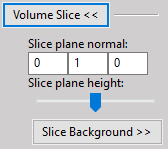
\includegraphics[width=\textwidth]{GUI/slice_collapsible.PNG}
    \caption{SliceControlCollapsible-objekt i fönster.}
  \end{minipage}
  \hfill
  \begin{minipage}[b]{0.4\textwidth}
    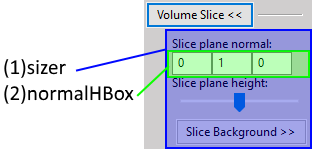
\includegraphics[width=\textwidth]{GUI/slice_collapsible_sizers.PNG}
    \caption{SliceControlCollapsible, sizer-struktur.}
  \end{minipage}
\end{figure}

Funktioner i klassen är callbacks för olika events som endast kör motsvarante funktion i  \textit{VolumeNetworkHandler}-objektet efter användarinteraktion.

\subsubsection{BackgroundCollapsible}
En kollapserbar meny för att styra en bakgrund i ett inviwonätverk. Används i både \textit{VolumeControlCollapsible} och \textit{SliceControlCollapsible} för att styra olika bakgrunder.

Klassen interagerar med ett \textit{VolumeNetworkHandler}-objekt för att kalla på funktioner för att ändra bakgrunder i de olika bilderna.

\textit{BackgroundCollapsible} låter en användare göra följande:
\begin{itemize}
    \setlength\itemsep{0em}
    \item Välja bakgrundsstil.
    \item Välja de två färgerna för bakgrundern.
    \item Byta plats på färgerna.
    \item Välja \textit{blend mode} för bakgrunden.
\end{itemize}

\nyBild{GUI/background_collapsible.PNG}{BackgroundCollapsible-objekt i fönster.}{BackgroundCollapsible}{1}

\textbf{BgColourWidget: } För att förenkla och abstrahera GUI-strukturen så har en klass BgColourWidget definerats. Widgeten en \textit{wx.ColourPicker} där en färg kan väljas. Den har även fyra textfält där en färg manuellt kan väljas från ett RGBA-värde. Klassen har även funktioner för att hämta ut och sätta värden i textfälten. Två \textit{BgColourWidget} används i \textit{BackgroundCollapsible} för att hantera de två färgerna i bakgrunden.

\nyBild{GUI/background_color.PNG}{BgColourWidget-objekt i fönster.}{BgColourWidget}{1}

\subsubsection{UnitcellCollapsible}
En kollapserbar meny för att styra en atompositionsaspekten av en visualisering. Denna används i både laddningstäthets- och i ELF-menyn (och bör även användas till partiell laddningstäthet då den läggs till i gränssnittet).

Klassen interagerar med ett \textit{UnitcellNetworkHandler}-objekt för att styra den del av inviwonätverket som är relevant. \textit{UnitcellCollapsible} initierar inte sin egen \textit{UnitcellNetworkHandler} utan variabeln \textit{networkHandler} måste sättas utifrån klassen innan den kan användas.

\newpage

\textit{UnitcellCollapsible} låter en användare göra följande:
\begin{itemize}
    \setlength\itemsep{0em}
    \item Välja radie för enskilda atomtyper.
\end{itemize}

\nyBild{GUI/unitcell_collapsible.PNG}{UnitcellCollapsible-objekt i fönster.}{UnitcellCollapsible}{1}

\textbf{UnitcellControlWidget: } För att förenkla och abstrahera GUI-strukturen så har en klass UnitcellControlWidget definerats. Widgeten består av en \textit{wx.StaticText} för att skriva atomnamnet och en \textit{wx.Slider} för att välja atomradie. Klassen interagerar med inviwonätverket via samma \textit{UnitcellNetworkHandler} som den \textit{UnitcellCollapsible} den är tillagd på.

\nyBild{GUI/unitcell_widget.PNG}{UnitcellControlWidget-objekt i fönster.}{UnitcellControlWidget}{1}

Då gränssnittet, och därmed \textit{UnitcellCollapible}-objektet, först initieras är inte en HDF5-fil än vald och ingen information om vilka atomslag som ska ingå i menyn finns. Funktionen \textit{add\_atom\_control} används därför. Funktionen lägger till ett \textit{UnitcellControlWidget}-objekt under menyn med ett definerat namn och index. Efter att en visualisering startas så kallas denna funktion för att lägga till alla atomer som visualiseringen innehåller.



\subsection{Parsningsmenyn}
Parser-systemet i ENVISIoN har inkorporerats i det grafiska gränssnittet. Detta förenklar användning av parsern då tillgång ges till alla parsning-skript genom kommandon på hög nivå. Filen där det grafiska gränssnittet har utvecklats heter $"$ParserPane.py$"$ När parsnings-menyn fälls ut, från start-fönstret, öppnas ett segment enligt figur \ref{fig:GUIParser}.

\begin{figure}[H]
  \centering
    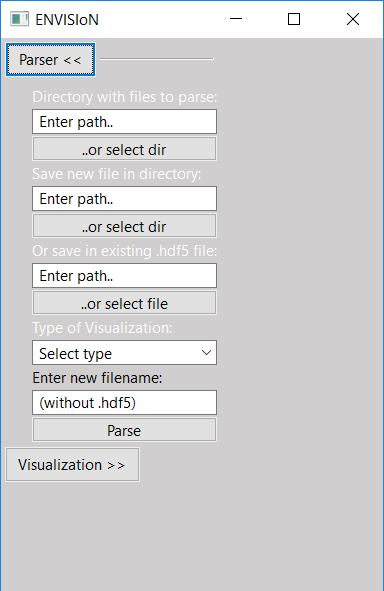
\includegraphics[scale=0.5]{images/GUI/GUIParserWin.png}
    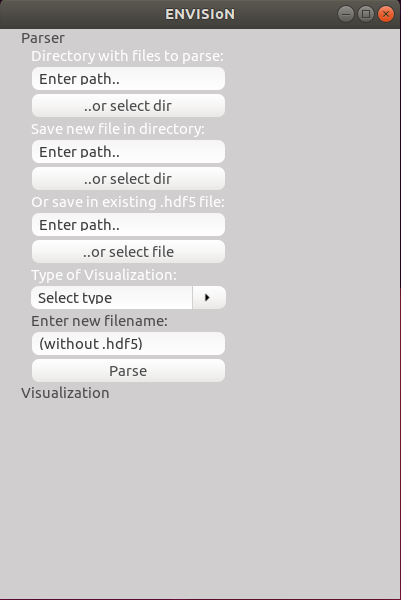
\includegraphics[scale=0.367]{images/GUI/GUIParserLinux.png}
    \caption{Parsermenyn i ENVISIoN, Windows till vänster och Linux till höger.}
    \label{fig:GUIParser}
\end{figure}

Överst i menyn väljs en mapp, innehållande relevanta beräkningsfiler, som önskas parsas. Detta går att välja genom att skriva sökvägen i textfältet, wx.TextCtrl, eller genom att trycka på $"$..or select dir$"$. Det senare alternativet öppnar en filhanterare som tillåter val av mapp.
På samma sätt väljs i nästa del en mapp att spara en ny hdf5-fil där parsningsresultatet lagras. För att spara en ny fil måste ett filnamn anges under rubriken $"$Enter new filename:$"$. Ett alternativ till detta är om det redan existerar en hdf5-fil där resultatet önskas sparas. För detta väljs antingen den filen med filhanteraren, under $"$..or select file$"$, eller genom att skriva sökvägen till filen i rutan tillhörande knappen.
En wx.ComboBox är tillagd som innehåller de parsningsval som är tillhandahållna av ENVISIoN. Dessa val innefattar:

\begin{itemize}
    \setlength\itemsep{0em}
    \item All
    \item Bandstructure
    \item Charge
    \item DoS - Density of States
    \item ELF - Electron Localization Function
    \item Fermi Energy
    \item MD - Molecular Dynamics
    \item Parchg - Partial Charge
    \item PCF - Pair Correlation Function
    \item Unitcell
\end{itemize}

När användaren är nöjd med sina val trycks parse-knappen längst ned och ett meddelande dyker upp på skärmen. Detta meddelande innehåller information om parsningen lyckades eller inte, och för vilken visualiserings-data parsningen lyckades, om den gjorde det.

\newpage

Det finns huvudsakligen en viktig funktion i parser-skriptet:

\begin{itemize}
    \item \textbf{parse\_pressed: }Den funktion där parsern aktiveras. Val av typ och lagringsval undersöks här. Här sker även felkontroll om parsningen lyckats eller inte.
\end{itemize}

Samtliga fält i parser-menyn som kan ändras har en kopplad funktion för händelse-hantering.

De filer som GUI:t kommunicerar med i parser-skriptet är:

\begin{itemize}
    \setlength\itemsep{0em}
    \item bandstructure.py
    \item doscar.py
    \item md.py
    \item unitcell.py
    \item volume.py
    \item fermi.py
    \item parchg.py
    \item PCF.py
    \item fermiEnergy.py
    \item main.py
\end{itemize}

Samtliga dessa filer, förutom $"$main.py$"$, finns i mappen $"$ENVISIoN/envision/envision/parser/vasp$"$, $"$main.py$"$ finns i $"$ENVISIoN/envision/envision$"$. Se appendix \ref{sec:GUIAppendix} för sökvägar relevanta för GUI:t.

\subsection{Visualiseringsmenyer}
Här beskriv de olika visuliseringsmenyernas uppbygnad och funktion.

\subsubsection{ChargeFrame}
En kollapserbar meny för att starta och styra en laddningstäthetsvisualisering. Har en \textit{VolumeControlCollapsible}, \textit{UnitcellCollapsible}, \textit{BackgroundCollapsible}, och \textit{SliceControlCollapsible} under sig tillsamans med kontroller för att välja band och aktivera slice och atomrendering.

Klassen tillgängliggör ett gränssnitt för användaren att interagera med ett \textit{ChargeNetworkHandler}-objekt.

\textit{ChargeFrame} låter en användare göra följande, utöver det som tillåts i dess underklasser:
\begin{itemize}
    \setlength\itemsep{0em}
    \item Starta och avsluta en visualisering (genom att fälla in och ut menyn).
    \item Välja aktivt atomband som ska visualiseras.
    \item Välja om atompositioner ska renderas eller inte.
    \item Välja om tvärsnitt ska visualiseras eller inte.
\end{itemize}


\nyBild{GUI/charge_collapsible_ex.PNG}{ChargeFrame i fönster.}{ChargeFrame}{1}

Speciella funktioner i \textit{ChargeFrame}:
\begin{itemize}
    \setlength\itemsep{0em}
    \item \textbf{on\_collapse: } Körs då ChargeFrame fälls ut eller ihop. 
    \begin{itemize}
        \setlength\itemsep{0em}
        \item Om menyn fälls ut så försöker den att starta en visualisering genom att initiera ett \textit{ChargeNetworkHandler}-objekt och att initiera dess undermenyer med detta. 
        
        Om visualiseringen misslyckas att startas så fälls menyn ihop igen och nätverket rensas.
        \item Om menyn fälls ihop så avslutas visualiseringen och nätverket rensas.
    \end{itemize}
    \item \textbf{reset\_canvas\_positions} Sätter visualiseringens canvas-position baserat på fönstrets position.
\end{itemize}


\subsubsection{ELFFrame}
ELFFrame är identisk jämfört med ChargeFrame med undantaget att en ELFNetworkHandler används istället för ChargeNetworkHandler samt titeln på menyn.

\subsubsection{ParchgFrame}
En kollapserbar meny för att starta och styra visualiseringen av partiell laddningstäthet. Har en \textit{VolumeControlCollapsible}, \textit{UnitcellCollapsible}, \textit{BackgroundCollapsible}, och \textit{SliceControlCollapsible} under sig tillsamans med kontroller för att välja aktiva band och lägen.

Klassen tillgängliggör ett gränssnitt för användaren att interagera med ett \textit{ParchgNetworkHandler}-objekt.

\textit{ParchgFrame} låter en användare göra följande, utöver det som tillåts i dess underklasser:
\begin{itemize}
    \setlength\itemsep{0em}
    \item Starta och avsluta en visualisering (genom att fälla in och ut menyn).
    \item Välja ett godtyckligt antal band som ska visualiseras.
    \item Välja om atompositioner ska renderas eller inte.
    \item Välja om tvärsnitt ska visualiseras eller inte.
\end{itemize}

\nyBild{GUI/parchg_collapsible_ex.png}{ParchgFrame i fönster.}{ChargeFrame}{1}

Speciella funktioner i \textit{ParchgFrame}:
\begin{itemize}
    \setlength\itemsep{0em}
    \item \textbf{on\_collapse: } Körs då ParchgFrame fälls ut eller ihop. 
    \begin{itemize}
        \setlength\itemsep{0em}
        \item Om menyn fälls ut så försöker den att starta en visualisering genom att initiera ett \textit{ParchgNetworkHandler}-objekt och att initiera dess undermenyer med detta. 
        
        Om visualiseringen misslyckas att startas så fälls menyn ihop igen och nätverket rensas.
        \item Om menyn fälls ihop så avslutas visualiseringen och nätverket rensas.
    \end{itemize}
    \item \textbf{reset\_canvas\_positions} Sätter visualiseringens canvas-position baserat på fönstrets position.
    \item \textbf{reload\_band\_processors} Läser valt band och läge i alla valda \textit{BandSelectorWidget} och sätter dessa som aktiva.
\end{itemize}

\subsubsection{2D-visualiseringar i grafer}
Visualiseringar i tvådimensionella grafer i ENVISIoN har många saker gemensamt. Detta har gjort att gränssnitten för dessa tre visualiseringar, bandstruktur, parkorrelationsfunktionen och tillståndstäthet, utvecklades på nästan identiskt vis. Det finns dock några skillnader.

\paragraph{BandstructureFrame} är klassen till den kollapsbara menyn för bandstrukturvisualiseringen. Figur \ref{fig:GUIBand} visar hur denna meny ser ut för både Windows och Linux. Under denna meny gömmer sig ett antal textfält och reglage.
\begin{figure}[H]
  \centering
    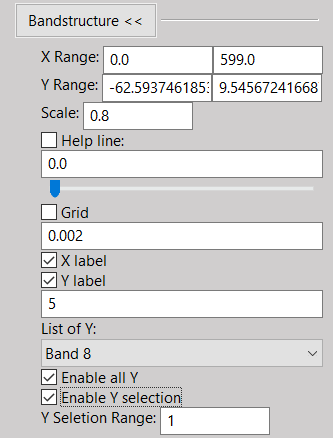
\includegraphics[scale=0.5]{images/GUI/GUIBandWin.png}
    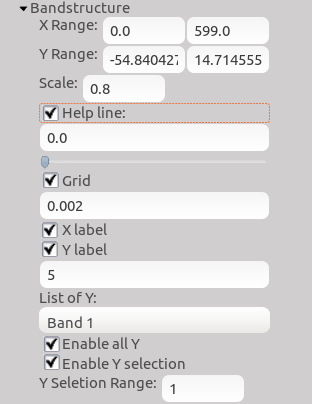
\includegraphics[scale=0.542]{images/GUI/GUIBandLinux.png}
    \caption{Visualiseringsmenyn för bandstruktur, Windows till vänster och Linux till höger.}
    \label{fig:GUIBand}
\end{figure}

\paragraph{PCFFrame} är klassen till den kollapsbara menyn för parkorrelationsfunktions-visualiseringen. Även figur \ref{fig:GUIPCF} visar hur denna meny ser ut för både Windows och Linux. Här syns tydligt hur lika menyerna för graf-visualiseringarna är vid jämförelse med bandstruktur-menyn.

\begin{figure}[H]
  \centering
    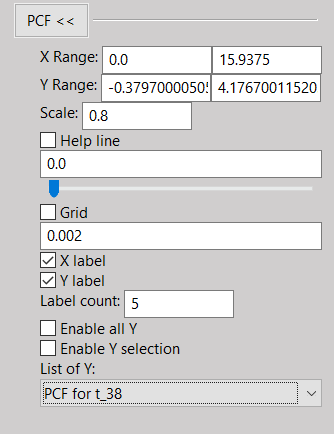
\includegraphics[scale=0.5]{images/GUI/GUIPCFWin.png}
    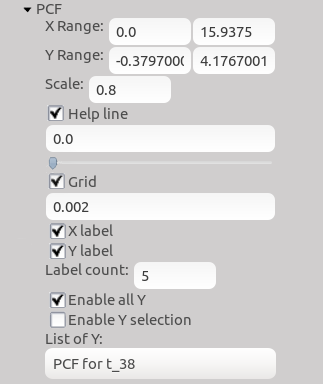
\includegraphics[scale=0.565]{images/GUI/GUIPCFLinux.png}
    \caption{Visualiseringsmenyn för parkorrelationsfunktionen, Windows till vänster och Linux till höger.}
    \label{fig:GUIPCF}
\end{figure}

\paragraph{DosFrame} är klassen till den kollapsbara menyn för tillståndstäthetvisualiseringen. Figur \ref{fig:GUIDoS} visar hur denna meny ser ut för Windows och Linux.

\begin{figure}[H]
  \centering
    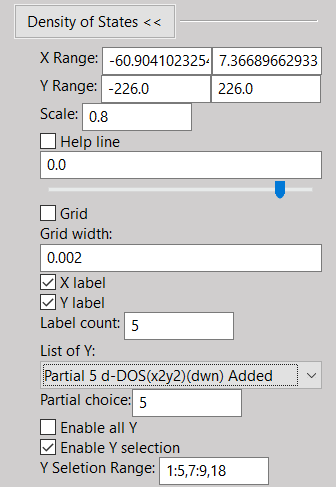
\includegraphics[scale=0.5]{images/GUI/GUIDoSWin.png}
    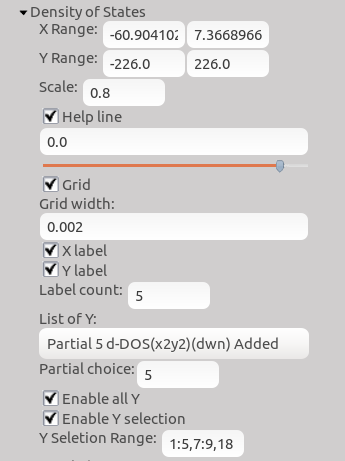
\includegraphics[scale=0.529]{images/GUI/GUIDoSLinux.png}
    \caption{Visualiseringsmenyn för tillståndstäthet, Windows till vänster och Linux till höger.}
    \label{fig:GUIDoS}
\end{figure}

\paragraph{Gemensamt för 2D-visualiseringar i graf} är uppbyggnad och till största del dess funktion, se figur \ref{fig:GUIBand}, \ref{fig:GUIPCF} och \ref{fig:GUIDoS}. Alla dessa meny-klasser är av typen GeneralCollapsible och ärver därför de funktioner som tillhör denna generella klass. Utöver detta har varje visualiseringsklass egna egenskaper. Det som är möjligt att ändra i dessa visualiserngar är:
\begin{itemize}
    \setlength\itemsep{0em}
    \item Ändra synligt intervall för båda axlarna genom att sätta minsta och största synliga värde i textboxarna, vänster respektive höger, vid $X Range$ och $Y Range$.
    \item Ändra skalningen för hela grafen genom att skriva ett decimaltal mindre än ett i rutan för $Scale$
    \item Aktivera eller inaktivera en hjälplinje. Denna hjälplinje kan flytta antingen med hjälp av manuell inmatning av x-värde i textrutan eller genom att dra i skjutreglaget. Vid flytt av skjutreglage uppdateras textrutan med det nya x-värdet där linjen placerats.
    \item Aktivera eller inaktivera ett rutnät. Detta rutnät är till för att, lättare, snabbt kunna läsa av värden på kurvan. Rutnätslinjernas tjocklek kan ändras genom att manuellt mata in ett värde mellan 0.0001 och 0.01 i textfältet under kryssrutan för $Grid$.
    \item Hantera etiketter utskrivna längs axlarna i grafen. Dels finns möjligheten av visa grafen både utan och med värden längs axlarna. Sedan finns även möjligheten att välja hur många sådan etiketter som skall finnas längs axlarna. Dessa placeras med jämna intervall från minsta synliga värde till största.
    \item Välja vilka linjer som skall visas i grafen. Det sista segmentet i visualiseringsfönstret för dessa visualiseringar handlar om val av data. Det visas för samtliga graf-visualiseringar, en lista med de data frames innehållande y-data som finns tillgängliga. Det finns två kryssrutor, en för att visa alla linjer och en för att välja en eller flera linjer. För att välja flera linjer kan intervall eller enstaka linjer väljas genom att skriva dess index i textrutan som öppnas när $Enable Y selection$ kryssas i.
\end{itemize}

\newpage

\paragraph{Skillnader mellan 2D-visualiseringar i graf} är att tillståndstäthetsvisualiseringen har en möjlighet att välja vilken partiell tillståndstäthet som önskas visualiseras. Detta genom att skriva in ett heltal i textrutan för $Partial pick$. För både tillståndstäthet och parkorrelationsfunktionen kan enstaka linjer väljas i listan av data frames, för bandstruktur är denna lista enbart en visuell lista. För visualisering av tillståndstäthet, i fallet att enhetscell-data finns tillgänglig hdf5-filen, öppnas ett extra fönster med enhetscellens visualisering.
\newline

Samtliga dessa funktioner kommunicerar med visualiseringsnätverket via funktioner från hjälpfilen paramterer\_utils.py, se kapitel \ref{sssec:paramUtils}.
Viktiga funktioner som är speciella för graf-visualiseringar är:
\begin{itemize}
    \setlength\itemsep{0em}
    \item \textbf{on\_collapse(self, event = None): } Aktiveras vid kollaps eller expansion av varje meny. Startar visualisering eller rensar nätverket.
    \item \textbf{start\_vis(self): }Kollar om rätt data finns i given hdf5-fil. Kallar på visuaiseringsskriptet eller skickar felmeddelande
    \item \textbf{init\_DoS(self), init\_bandstructure(self) och init\_PCF(self): } Sätter alla parametrar i GUI:t till de som visualiseringen startas med.
\end{itemize}

Utöver dessa finns det funktioner som är kopplade till de element som är synliga i GUI:t och har en funktion att styra en egenskap hos visualiseringen.

\subsection{Inviwointeraktion}
För att interagera med inviwonätverket och påverka visualiseringarna så används två olika tilvägagångssätt. För de visualiseringar där \textit{NetworkHandler}-klasser finns definerade så används dessa. Se kapitel \ref{ssec:NetworkHandlers}. För återstående visualiseringar, PCF, DOS, och Bandstruktur, så används funktioner i en fil ''parameter\_utils.py'' för att interagera med inviwonätverket.


\subsubsection{parameter\_utils.py}\label{sssec:paramUtils}
Filen parameter\_utils.py innehåller funktioner som sköter kommunikaton med olika processorer i nätverket. Det generella strukturen på dessa funktioner är att de tar en processoridentitet i form av en sträng. I de fall att ett värde skall sättas är även detta värde en parameter. De funktioner som finns i denna fil hanterar till exempel fönsterposition för det fönster visualiseringarna öppnas i. I denna fil finns även funktinerna till styrning av parameterar i lineplotprocessorn som är relevanta för de, i GUI:t, existerande visualiseringarna. 
Viktiga funktioner som finns i parameter\_utils är:
\begin{itemize}
    \setlength\itemsep{0em}
    \item \textbf{clear\_processor\_network(): }Rensar arbetsytan från processorer.
    \item \textbf{change\_scale(scaleValue,processor='Line plot'): }Ändrar skalningen av grafen i lineplotprocessorn
    \item \textbf{set\_all\_data(processor='',setAll=True): }Sätter om alla linjer skall visas i grafen.
    \item \textbf{set\_yline\_range(option=1,processor='Line plot'): }Sätter vilka linjer, en eller flera, som skall ritas ut i grafen.
    \item \textbf{choose\_line(index=1,processor='Line plot'): }Sätter vilken linje, endast en, som skall visas i grafen.
    \item \textbf{set\_x\_range(value, type, processor='Line plot'): }Sätter vilket intervall som skall vara synligt på x-axeln.
    \item \textbf{set\_y\_range(value, type, processor='Line plot'): }Sätter vilket intervall som skall vara synligt på y-axeln.
    \item \textbf{set\_help\_line(value, processor='Line plot'): }Sätter var hjälp-linjen skall vara.
    \item \textbf{set\_grid(value=None,processor='Line plot'): }Sätter tjockleken på rutnätets linjer.
    \item \textbf{set\_canvas\_position(position = None, processor='Canvas'): }Sätter visualiseringsfönstrets position.
    \item \textbf{set\_label(value=None,processor='Line plot'): }Sätter hur många värden som ska skrivas ut på axlarna, borträknat minsta värdet.
    \item \textbf{set\_partial\_value(option=1,processor='Line plot'): }För tillståndstäthet sätter denna funktion vilken partiell täthet som skall visas.
\end{itemize}

Samtliga funktioner i parameter\_utils.py som sätter ett värde har en motsvarande funktion som hämtar det värdet som vid tillfället är satt. Samtliga dessa funktioner är namngivna med stilen $"$get\_[vad som ska hämtas]$"$ till exempel $"$get\_scale$"$.

